\documentclass[journal, onecolumn, a4paper]{IEEEtran}

\usepackage{graphicx} 
\usepackage{url}
\usepackage{amsmath}
\usepackage[utf8]{inputenc}
\usepackage[main=english, czech]{babel}
\usepackage{mathtools}
\usepackage{subfigure}
\newcommand*{\Scale}[2][4]{\scalebox{#1}{$#2$}}%
\newcommand*{\Resize}[2]{\resizebox{#1}{!}{$#2$}}%
\setlength{\parskip}{0.25em}

\renewcommand{\IEEEbibitemsep}{0pt plus 0.5pt}
\makeatletter
\IEEEtriggercmd{\reset@font\normalfont\fontsize{7.9pt}{8.40pt}\selectfont}
\makeatother
\IEEEtriggeratref{1}

% Your document starts here!
\begin{document}

\setlength{\abovedisplayskip}{0pt}

% Define document title and author
	\title{Computer-Aided Spatial Planning and Design - Mask R-CNN}
	\author{Ondřej Pešek}
	\markboth{National Cheng Kung University, Tainan}{}
	\maketitle

% Write abstract here
\begin{abstract}
The usage of artificial neural networks in the geomatics field is really wide. 
One of the most requested applications is the classification of satellite 
images. Among many different approaches, I have chosen Mask R-CNN (region-based 
convolutional neural networks) proposed by Facebook AI Research as our 
framework, allowing user to both detect objects and generate a segmentation mask 
for each instance. 

\end{abstract}

% Each section begins with a \section{title} command
\section*{Introduction}

\IEEEPARstart{A}{rtificial} neural network. A magical formula that can be heard more and more often in almost every part of computer science. Computing systems with many applications in finance, data mining, language recognition, pattern recognition and many more. With the last named are connected attempts to use artificial neural networks in geomatics field for an automated classification of satellite images. 

Classification is a separation of regions of interest. Artificial neural networks allowed two approaches for classification so far (following the terminology from \cite{mask-rcnn}):
\begin{itemize}
\item \textbf{Object detection}: Detecting objects via bounding boxes, for example \cite{objectdet}
\item \textbf{Semantic segmentation}: Per-pixel classification of whole image without assigning pixels to different instances, for example those used in remote sensing \cite{fcnn-seg}
\end{itemize}

Mask region-based convolutional neural networks (Mask R-CNN) proposed by 
Facebook AI Research provides a combination of both approaches - object 
detection via bounding boxes and following semantical segmentation of bounded 
area. As we are segmenting the detected instance, this process is called 
instance segmentation and could be useful in satellite images classification. 


The goal of this paper is to give an insight into Mask R-CNN and artificial neural networks generally and discuss and design its implementation in geomatics field. 

\section{Prerequisites}
\label{history}

\IEEEPARstart{S}{peaking} generally, Mask R-CNN are just Faster R-CNN \cite{faster-rcnn} with one additional layer for the mask (and few smaller changes). Considering that, I should firstly talk about Faster R-CNN and other related terms before explaining Mask R-CNN specifications in chapter \ref{network}.

% \subsection{CNN}

\subsection{R-CNN}
\label{subsec:rcnn}

R-CNN is an acronym for region-based convolutional neural networks, an algorithm proposed in \cite{rcnn} and combining region proposals with convolutional neural networks to detect objects in image via bounding boxes.  

The first step of detection is to propose bounding boxes using the selective search \cite{search} - an algorithm consisting of two steps: 
\begin{itemize}
\item \textbf{All scales capturing}: Generating many bounding boxes (region proposals) at different scales based on their texture, color or intesity similarities. An hierarchical algorithm is used. 
\item \textbf{Group regions together}: Grouping is influenced by colors, shades and other natural and non-natural conditions. To reduce these influences, a diverse set of strategies is held. 
\end{itemize}

After bounding boxes proposition we have to compute region features. This requires warping the region into 227 x 227 square RGB image, which can be forward propagated through an architecture composed of five convolutional layers and two fully connected layers (modified architecture described in \cite{cnn-class}). 

The final step is scoring of those extracted features (deciding which class the feature is and whether it is any class at all). This is done for each feature separately using a Support Vector Machine (SVM) trained for that class. 

In general, the bounding box has a large overlap with the background. This is the last problem with which the algorithm has to deal. To improve the localization (make bounding boxes tighter), a bounding box regression proposed in \cite{bbox-regression} is used with one modification - R-CNN applies regression on features computed by the CNN instead of features computed on the inferred deformable part model (DPM) locations. 

\begin{figure}[h] \centering
	\includegraphics[width=0.9\textwidth]{rcnn}
	\caption{R-CNN architecture, source: \cite{rcnn}}
\end{figure}

Although R-CNN outperformed similar architectures including OverFeat (according to \cite{rcnn}), there were still some shortcomings. The biggest one was the slowness caused mainly by the forward propagation through CNN (each region of every image must be passed separately), by its triplicated training (a network for generating image features, a network for the class decision and the bounding box regression model) and by the generating of bounding box proposals. Then, in year 2015, Fast R-CNN came to solve first two of these issues. Lead by the author of original R-CNN, Ross Girshick. 

\subsection{Fast R-CNN}

Because the main reason for a new architecture was to speed-up R-CNN, Ross Girshick named his new architecture proposed in \cite{fast-rcnn} simply Fast R-CNN. Its main purposes were to avoid first two issues mentioned in chapter \ref{subsec:rcnn} and improve its accuracy. 

The first issue, the separate forward propagations, was solved by propagating the entire image and the full set of its object proposals through a set of convolutional and max pooling layers. For each object proposal is then from the feature map extracted a fixed-length feature vector by a region of interest (RoI) pooling layer. The RoI pooling layer can be seen as a one level spatial pyramid pooling layer, a max pooling based downsampling algorithm proposed in \cite{SPP}, and its purpose is to decompose separately each valid region of interest into a fixed size (7 $\times$ 7) grid, where each cell represents a feature map. The RoIPool decomposition is made by quantization a RoI to the rounded discrete granularity of the feature map which is then (again with quantization) divided into 7 $\times$ 7 bins. Final values of each bin are aggregated by max pooling. 

Output of RoI pooling layers is an input for a sequence of fully connected layers. Then the last, branched step where two different outputs are obtained depending on the last layer - class probabilities from a softmax function and a bounding box defined by 4 values from a regressor. 

There can be seen also a solution of the second problem named in \ref{subsec:rcnn}. Instead of three separate models, all steps are joint into only one model by appending classification (using a softmax layer instead of a separate SVM) and bounding box regression as parallel layers to the end of the model. 

\begin{figure}[h] \centering
	\includegraphics[width=0.9\textwidth]{fastrcnn}
	\caption{Fast R-CNN architecture, source: \cite{fast-rcnn}}
	\label{fig:fast-rcnn}
\end{figure}

There can be raised a question whether is the SVM replacement with the softmax layer as accurate as the original approach. According to tests performed in \cite{fast-rcnn}, the softmax layer is even slightly outperforming SVM. 

\subsection{Faster R-CNN}

The third speed issue mentioned in chapter \ref{subsec:rcnn} - the region proposer based on the selective search - was solved in year 2016 in an architecture imaginatively named Faster R-CNN, proposed in \cite{faster-rcnn}. 

Microsoft Research team found that feature map computed in the first part of Fast R-CNN can be used to generate region proposals instead of using slower selective search algorithm. This is done by including Region Proposal Network (RPN) consisting of a few convolutional layers (a fully convolutional network) after the convolutional feature maps of Fast R-CNN. The RPN layer backbone are two fully connected layers, one for a bounding box regression and one for a bounding box classification. The complete architecture alternates between fine-tuning for the region proposal task and for the object detection. This approach with shared convolutional features quickly converges. 

\begin{figure}[h] \centering
	\includegraphics[width=0.55\textwidth]{fasterrcnn}
	\caption{Faster R-CNN architecture, source: \cite{faster-rcnn}}
\end{figure}

RPN approach is different than the ones used in other architectures. Instead of pyramids of images or filters, RPN uses anchor boxes - a set of rectangular bounding boxes proposals and scores created by sliding a spatial window over the entire convolutional feature map. Those anchors are defined by a scale and aspect ratio, so they are of different shapes. Powerful attributes of anchors are that they are translation-invariant and multi-scale, which concludes also into a reduction of the model size. 

\begin{figure}[h] \centering
	\includegraphics[width=0.5\textwidth]{fasterrcnn-anchors}
	\caption{Region Proposal Network, source: \cite{faster-rcnn}}
\end{figure}

\section{Mask R-CNN}
\label{network}

\IEEEPARstart{S}{o} we had R-CNN, Fast R-CNN and Faster R-CNN. What could be the next step? The first answer that comes to your mind is wrong - instead of expected \textit{The Fastest R-CNN}, the Mask R-CNN were proposed in year 2017 by Facebook AI Research (FAIR) in \cite{mask-rcnn}. 

FAIR stood in a front of another question. According to \cite{faster-rcnn}, Faster R-CNN outperformed most of their concurrents in the object detection. But it was still unusable for some users looking for a semantic segmentation neural network. They had a powerful network for object detection, so the question was: Is there any way to use the current network for the semantic segmentation? 

Obviously, the answer was - yes. But instead of the semantic segmentation, they proposed more advanced approach, the instance segmentation, which was described in the introduction of this paper and in \cite{mask-rcnn}. An approach that provides much richer usage in geomatics field. 

To implement the instance segmentation with sufficient accuracy, there was a need for some changes in the architecture of Faster R-CNN. Following the original terminology from \cite{mask-rcnn}, in the following part, I will distinguish between the backbone architecture for feature extraction and the head architecture for classification, bounding box regression and mask prediction. Those will be described in the following parts of this chapter along with an extra focus on some other major changes. 

\begin{figure}[h] \centering
	\includegraphics[width=0.4\textwidth]{maskrcnn}
	\caption{Mask R-CNN architecture, source: \cite{mask-rcnn}}
	\label{fig:mask-rcnn}
\end{figure}

\subsection{Backbone architecture}

For the backbone architecture, more architectures can be used, but in the original paper \cite{mask-rcnn}, ResNet (residual network) was used. ResNet is a deep neural network oriented residual framework with layers reformulated as learning residual functions with reference to the layer inputs proposed in \cite{resnet}. ResNet provides frameworks of various depth - ResNet-20, ResNet-32, ResNet-50, ResNet-101 and ResNet-152 where the number suffix represents a number of layers. In \cite{resnet}, even network with more than 1000 layers was proposed, but it is not recommended to use such an extreme solution as its testing result was surprisingly worse than the that of 110 layer network (most likely because of overfitting). 

Moreover, the ResNet based backbone was extended by FPN (Feature Pyramid Network), a top-down architecture with lateral connections developed for building high-level semantic feature maps at different scales proposed in \cite{fpn}. FPN uses the fact that deep convolutional network computes a feature hierarchy layer by layer. By subsampling these layers, we can obtain a different spatial resolution feature hierarchy with multi-scale, pyramidal shape. To achieve strong semantics at all scales, FPN uses bottom-up, top-down pathways and lateral connections to create predictions independently on each level. The feature hierarchy is created by propagating a single scale image through the convolutional network (bottom-up pathway). Because each stage of the network outputs a map of the same size, one level of the FPN is created from output of the last layer of each stage except of the first stage due to its memory claims. The top-down pathway is done by upsampling feature maps from higher levels by a factor of 2 and using nearest neighbour upsampling, and then enhancing them via lateral connections with features from the bottom-up pathway as can be seen in figure \ref{fig:top-down}. 

\begin{figure}[h] \centering
	\includegraphics[width=0.4\textwidth]{top-down}
	\caption{A top-down architecture generating the feature pyramid, source: \cite{fpn}}
	\label{fig:top-down}
\end{figure}

\subsection{Head architecture}

In the head architecture, there was the most important change to allow the instance segmentation - including the mask branch in parallel with branches for classification and bounding box regression. 

The mask branch is a pixel-to-pixel FCN predicting a mask individually for each RoI, where mask is a binary matrix of ones (object location) and zeros (elsewhere). 

In figure \ref{fig:mask-rcnn-head}, we can see two implementations of the head architecture. The left one is based on ResNet-C4 (4 stage ResNet) and extends it with the compute intensive fifth stage, the right one is based on FPN which already includes the fifth stage. In these implementations, the last convolution is 1 $\times$ 1 and the other ones are 3 $\times$ 3 and are the ones with preserved shapes; deconvolutions are 2 $\times$ 2 with stride 2 and increase shapes. 

\begin{figure}[h] \centering
	\includegraphics[width=0.7\textwidth]{maskrcnn-head}
	\caption[caption]{\tabular[t]{@{}l@{}}Head architecture, source: \cite{mask-rcnn} \\ \textit{Left:} Extended Faster R-CNN with ResNet. \textit{Right:} Extended Faster R-CNN with FPN \endtabular}
	\label{fig:mask-rcnn-head}
\end{figure}

\subsection{Loss function}

Because there are three individual tasks (bounding box regression, classification, mask), the loss function $L$ is defined as a summation of individual loss functions: 

\begin{gather*}
L = L_{cls} + L_{box} + L_{mask}
\end{gather*}

$L_{cls}$ and $L_{box}$ are the same as in \cite{fast-rcnn}:

\begin{gather*}
L_{cls} = - log(p_u)
\end{gather*}
where:

$p_u$ is a probability of predicting the right class $u$,\\
and

\begin{gather*}
L_{box} = \sum\limits_{i \in \{x, y, w, h\}} smooth_{L_1}(t_i^u - v_i)\\
smooth_{L_1}(x) = \begin{cases}
	0.5 x^2 & \quad \text{if } |x| < 1\\
	|x| - 0.5 & \quad \text{otherwise}
\end{cases}
\end{gather*}
where:

$v$ is a tuple of ground-truth bounding box targets for class $u$ ($v_x$ for a $x$ coordinate, $v_y$ for an $y$ coordinate, $v_w$ for a width, and $v_h$ for a height of the box),

$t^u$ is a tuple of predicted bounding box targets for class $u$ ($t_x^u$, $t_y^u$, $t_w^u$, $t_h^u$).\\ 

A mask of resolution $m \times m$ is generated for each of the $K$ classes, so an output of the mask branch for each RoI is $K m^2$ dimensional. Mask loss $L_{mask}$ was defined in \cite{mask-rcnn} as the average binary cross-entropy loss of a per-pixel sigmoid function applied to the output of positive RoIs. This approach means that each mask is generated without competing with the others relying on the prediction of class label to select the right one. This is different from a common approach using per-pixel softmax function and a multinomial cross-entropy loss and according to experiments provided by \cite{mask-rcnn}, the decoupled prediction gives better results in instance segmentation. 

\subsection{RoIAlign}

In figure \ref{fig:mask-rcnn}, we can see a RoIAlign layer instead of Fast R-CNN RoIPooling from figure \ref{fig:fast-rcnn}. 

This change was needed because of spatial inaccuracy of RoIPool due to the fact that it was not intended to be used for a pixel-to-pixel alignment. This inaccuracy is caused by quantizations and roundings and RoIAlign avoids it simply by skipping the rounding. To compute the value of the input, a bilinear interpolation at regular sampled locations (usually 4) is used. 

According to \cite{mask-rcnn}, RoiAlign improved Mask R-CNN mask accuracy by relative 10 \% to 50 \%. 

\ 

\ 

\ 

\ 

\section{Geomatics field}

\IEEEPARstart{I}{n} remote sensing we are dealing with huge amount of satellite photos. Though there are many algorithms for an automated classification, there is one promising child which is just growing up and hogging the limelight. This child is called artificial neural networks. 

Artificial neural networks for image processing are very strong in an object detection. The object detection in aerial photos could be very useful for example for detecting sick trees in a forest image or for a vehicle detection (airplane, ship, car, etc.). In the world of geographical information systems (GIS), it means elements that can be represented as points. But what about searching for forests? Searching for lakes? Rivers? Oil spills? Do we really want to represent them in GIS as points in their center of mass? 

It seems that better representation is in polygons (or lines). But epresenting a detection bounding box as a polygon square does not seem like the right way. So there is the instance segmentation - generating a mask of instances that can be transformed into vector polygons or lines. 

\subsection{Implementation}

\begin{figure}[h] \centering
	\includegraphics[scale=0.9]{grass-logo}
	\caption{GRASS GIS logo, source: https://grass.osgeo.org/download/logos/}
	\label{fig:grass-logo}
\end{figure}

For our implementation, I have decided for GRASS (Geographic Resources Analysis Support System) GIS. GRASS GIS is a multi-platform GIS used for management, analysis, modeling and visualization of spatial data and images. Since GRASS GIS is an open-source software (GNU GPL license), implementing it into this software can provide it to many users. GRASS GIS also contains a lot of modules that can be used to fasten the vectorization and final data cleaning and is also computably fast, that is why GRASS GIS was chosen instead of other open-source GIS like QGIS. 

Our implementation was written in Python. There are few reasons for this: 
\begin{itemize}
\item Although some GRASS GIS modules are written in C and C++, most of them is written in Python.
\item Python allows us to use libraries such as TensorFlow\footnote{https://www.tensorflow.org/} and Keras\footnote{https://keras.io/}. 
\end{itemize}

Our code is based on a Python3 implemetation of Mask R-CNN by Matterport, Inc\footnote{https://matterport.com/}., written by Waleed Abdulla. I used files \verb|model.py| including the model using ResNet101 as its backbone and \verb|parallel_model.py| enabling the multi-GPU training from the Matterport official repository\footnote{https://github.com/matterport/Mask\_RCNN}. This code was published under open MIT license permitting us to use it and modify the code, and Abdulla himself also granted us the permission. \verb|parallel_model.py| was used in its original version, \verb|model.py| was modified, and the rest of code was written by us. 

One is allowed to choose his preferred option - train the network from the scratch or use a pre-trained network. Because training from the scratch is time consuming and the latter is in most cases sufficient, I included pre-trained weights trained on MS COCO\footnote{http://cocodataset.org/} provided by Matterport. For our usage it is recommended to use the pre-trained weights for RGB images, otherwise it is recommended to start the training from the scratch. 

With the preferred option is connected also another feature - a possibility to train your network in three steps. The first step trains only \textit{heads}, the second one fine-tunes ResNet stage 4 and higher and the last step all layers. This approach prefer training of new weights at the expense of the pre-trained ones in the beginning of the process and seems to allow faster training for images not greatly different from the ones used for pre-training. 

Training must be done on 3-band images with masks, where mask is provided for each instance separately. It means that if you want to train classes \verb|soccer|, \verb|tennis| and \verb|golf| and you have image \verb|tainan-01.jpg| containing two instances of soccer fields and one of a tennis field, you have to provide three masks \verb|tainan-01-soccer-0.png|, \verb|tainan-01-soccer-| \verb|1.png| and \verb|tainan-01-tennis-0.png|. These image-mask sets should be contained in separate folders (a logical one for this example should be \verb|tainan-01|) inside of a training folder. For the best precision, all training images should be in the same resolution as images on which I would like to use the network. 

Code may be seen at our Github repository\footnote{https://github.com/ctu-geoforall-lab-projects/dp-pesek-2018}. 

\subsection{Results}

The training dataset was created by using OpenStreetMap\footnote{https://www.openstreetmap.org/} and Bing Maps\footnote{https://www.bing.com/maps}. I downloaded ortophoto tiles and clipped them using query selecting \verb|soccer| (but I prefer to call it \textit{football} in the text, sorry) and \verb|tennis| fields from layer \verb|sports| from OpenStreetMaps. This clip was then transformed into a binary mask separately for each instance. 

Our training was stopped after 235 epochs, each consisting of 1500 steps. As I used weights pre-trained on MS COCO dataset provided by Matterport, Inc., I divided our training into 3 steps: 40 epochs of heads training, 60 epochs of fine-tuning with ResNet stage 4+ and 135 epochs of fine-tuning all layers, while the learning rate (0.001) was divided by 10 in the second step and by 100 in the last step. The training was stopped when the total loss oscilated for a long time (several epochs) around 0.58. 

Results of testing on a random sample of images not seen by the network (instead of USA I used Prague where I am more competent for considering the correctness) can be seen in the following table. There are percents for correctly recognized fields, for considering another field as a searched field and for not recognizing the searched field. Statistics were made on images with the same resolution as training images and on images with a halved revolution. 

\begin{tabular}{|r | c | c | c | c | c | c|}
	\hline
	\textbf{Type of field} & \multicolumn{2}{c |}{\textbf{Correctly recognised [\%]}} & \multicolumn{2}{c |}{\textbf{Labeled another field [\%]}} & \multicolumn{2}{c |}{\textbf{Not labeled [\%]}} \\
	& \textbf{Same resolution as training} & \textbf{Halved resolution} & \textbf{Same} & \textbf{Halved} & \textbf{Same} & \textbf{Halved}\\
	\hline
	Tennis & 99 & 97 & 0 & 0 & 1 & 3 \\
	\hline
	Football & 80 & 60 & 15 & 20 & 5 & 20 \\
	\hline
\end{tabular}

Figures illustrating the results visually can be seen in the appendix. 

Although I consider the results for tennis fields satisfying, the poor results in football fields are quite disappointing. This can be caused by the fact that some fields are not included in OSM and they are considered as non-target during the training. OSM areas does not also always fit exactly to the field from Bing tile. These facts affect both tennis and football fields, but another one does not - while tennis fields are mostly very professional, football fields are not. And football fields made on a meadow just by erecting two goals are the cause for considering empty fields as football fields. 

\section*{Conclusion}

I reviewed Mask R-CNN and the evolution concluding in this framework and I implemented it into an application (which I find as the best possible review). Although I find it very powerful and it allows user to both detect and segment the instance with satisfying results after a training in a tolerable time, my results were sometimes unsatisfying. 

However, I believe that using better training dataset can raise the accuracy in really stunning way. Another improvement could be using another architecture for the mask head branch, where I am currently using very basic one. Also when we look at chapter \ref{history}, we can see the huge progress made within 3 years and I am not afraid to say: Future promises more than ever! 

%*** Missing: Technologies (TF, Keras, Python, GRASS GIS) ***

%*** Input design (introduction?), training algorithm ***

%*** ResNet, ReLU v headu ***

% Now we need a bibliography:
\newpage
\begin{thebibliography}{5}

	%Each item starts with a \bibitem{reference} command and the details thereafter.
	%\bibitem{HOP96} % Transaction paper
	%J.~Hagenauer, E.~Offer, and L.~Papke. Iterative decoding of binary block
	%and convolutional codes. {\em IEEE Trans. Inform. Theory},
	%vol.~42, no.~2, pp.~429–-445, Mar. 1996.

	%\bibitem{Proakis} % Book
	%J.~G.~Proakis. {\em Digital Communications}. McGraw-Hill Book Co.,
	%New York, USA, 3rd edition, 1995.

	\bibitem{search} % Conference paper
	Uijlings J. R. R., van de Sande K. E. A., Gevers T. Selective Search for Object Recognition. {\em International Journal  of Computer Vision 104}, %Istanbul, Turkey,
	pp.~154--171, April 2013.

	\bibitem{cnn-class} % Conference paper
	Krizhevsky A., Sutskever I., Hinton G. E. Imagenet classification with deep convolutional neural networks. {\em Advances in neural information processing systems}, %Istanbul, Turkey,
	pp.~1097--1105, 2012.

	\bibitem{SPP} % Conference paper
	He K., Zhang X., Ren S., Sun J. {\em Spatial Pyramid Pooling in Deep Convolutional Networks for Visual Recognition}. ECCV 2014.
	\url{https://arxiv.org/abs/1406.4729}.

	\bibitem{objectdet} % Web document
	Huang J, Rathod V, Sun C, Zhu M, Korattikara A, Fathi A, Fischer I, Wojna Z,
Song Y, Guadarrama S, Murphy K. {\em Speed/accuracy trade-offs for modern convolutional object detectors}. CVPR 2017.
	\url{https://arxiv.org/abs/1703.06870}.

	\bibitem{fcnn-seg} % Web document
	Kemker R., Salvaggio C., Kanan Ch. {\em Algorithms for Semantic Segmentation of Multispectral Remote Sensing Imagery using Deep Learning}. CoRR 2017.
	\url{https://arxiv.org/abs/1703.06452}.

	\bibitem{bbox-regression} % Web document
	Felzenszwalb P. F., Girshick R., McAllester D., Ramanan D. {\em Object detection with discriminatively trained part based models}. IEEE Vol. 32 Issue 9, 2009.

	\bibitem{rcnn} % Web document
	Girshick R., Donahue J., Darrell T., Malik J. {\em Rich feature hierarchies for accurate object detection and semantic segmentation}. Computer Vision and Pattern Recognition. 2014. 
	\url{https://arxiv.org/abs/1311.2524}.

	\bibitem{fast-rcnn} % Web document
	Girshick R. {\em Fast R-CNN}. Computer Vision and Pattern Recognition. 2015.
	\url{https://arxiv.org/abs/1504.08083}.

	\bibitem{faster-rcnn} % Web document
	Ren S., He K., Girshick R., Sun J. {\em Faster R-CNN: Towards Real-Time Object Detection with Region Proposal Networks}. Advances in Neural Information Processing Systems. 2015.
	\url{https://arxiv.org/abs/1506.01497}.

	\bibitem{mask-rcnn} % Web document
	He K., Gkioxari G., Dollár P., Girshick R. {\em Mask R-CNN}. CoRR. March 2017.
	\url{https://arxiv.org/abs/1703.06870}.

	\bibitem{resnet} % Web document
	He K., Zhang X., Ren S., Sun J. {\em Deep Residual Learning for Image Recognition}. CoRR. December 2015.
	\url{https://arxiv.org/abs/1512.03385}.

	\bibitem{fpn} % Web document
	Lin T., Dollár P., Girshick R., He K., Hariharan B. Belongie S. {\em Feature Pyramid Networks for Object Detection}. CoRR. December 2016.
	\url{https://arxiv.org/abs/1612.03144}.

	\bibitem{rcnn2mask} % Web document
	Parthasarathy D. {\em A Brief History of CNNs in Image Segmentation: From R-CNN to Mask R-CNN}. Athelas.
	\url{https://blog.athelas.com/a-brief-history-of-cnns-in-image-segmentation-from-r-cnn-to-mask-r-cnn-34ea83205de4}.

\end{thebibliography}

\newpage
\appendices

\section{Image attachment}

\begin{figure}[h]
\hfill
\subfigure[GUI of my module ann.maskrcnn.train]{\includegraphics[width=.45\linewidth]{15}}
\hfill
\subfigure[GUI of my module ann.maskrcnn.train]{\includegraphics[width=.45\linewidth]{16}}
\hfill
\end{figure}

\begin{figure}[h]
\hfill
\subfigure[GUI of my module ann.maskrcnn.detect]{\includegraphics[width=.45\linewidth]{18}}
\hfill
\subfigure[GUI of my module ann.maskrcnn.detect]{\includegraphics[width=.45\linewidth]{19}}
\hfill
\end{figure}

\begin{figure}[h]
\hfill
\subfigure[Original image]{\includegraphics[width=.35\linewidth]{output4}}
\hfill
\subfigure[Masked image. The left mask could fit better]{\includegraphics[width=.35\linewidth]{output4_mask}}
\hfill
\end{figure}

\begin{figure}[h]
\hfill
\subfigure[Original image]{\includegraphics[width=.4\linewidth]{output5}}
\hfill
\subfigure[GRASS output]{\includegraphics[width=.4\linewidth]{1}}
\hfill
\end{figure}

\begin{figure}[h]
\hfill
\subfigure[Original image]{\includegraphics[width=.4\linewidth]{output4}}
\hfill
\subfigure[GRASS output]{\includegraphics[width=.4\linewidth]{2}}
\hfill
\end{figure}

\begin{figure}[h]
\hfill
\subfigure[Georeferenced tiles and polygons]{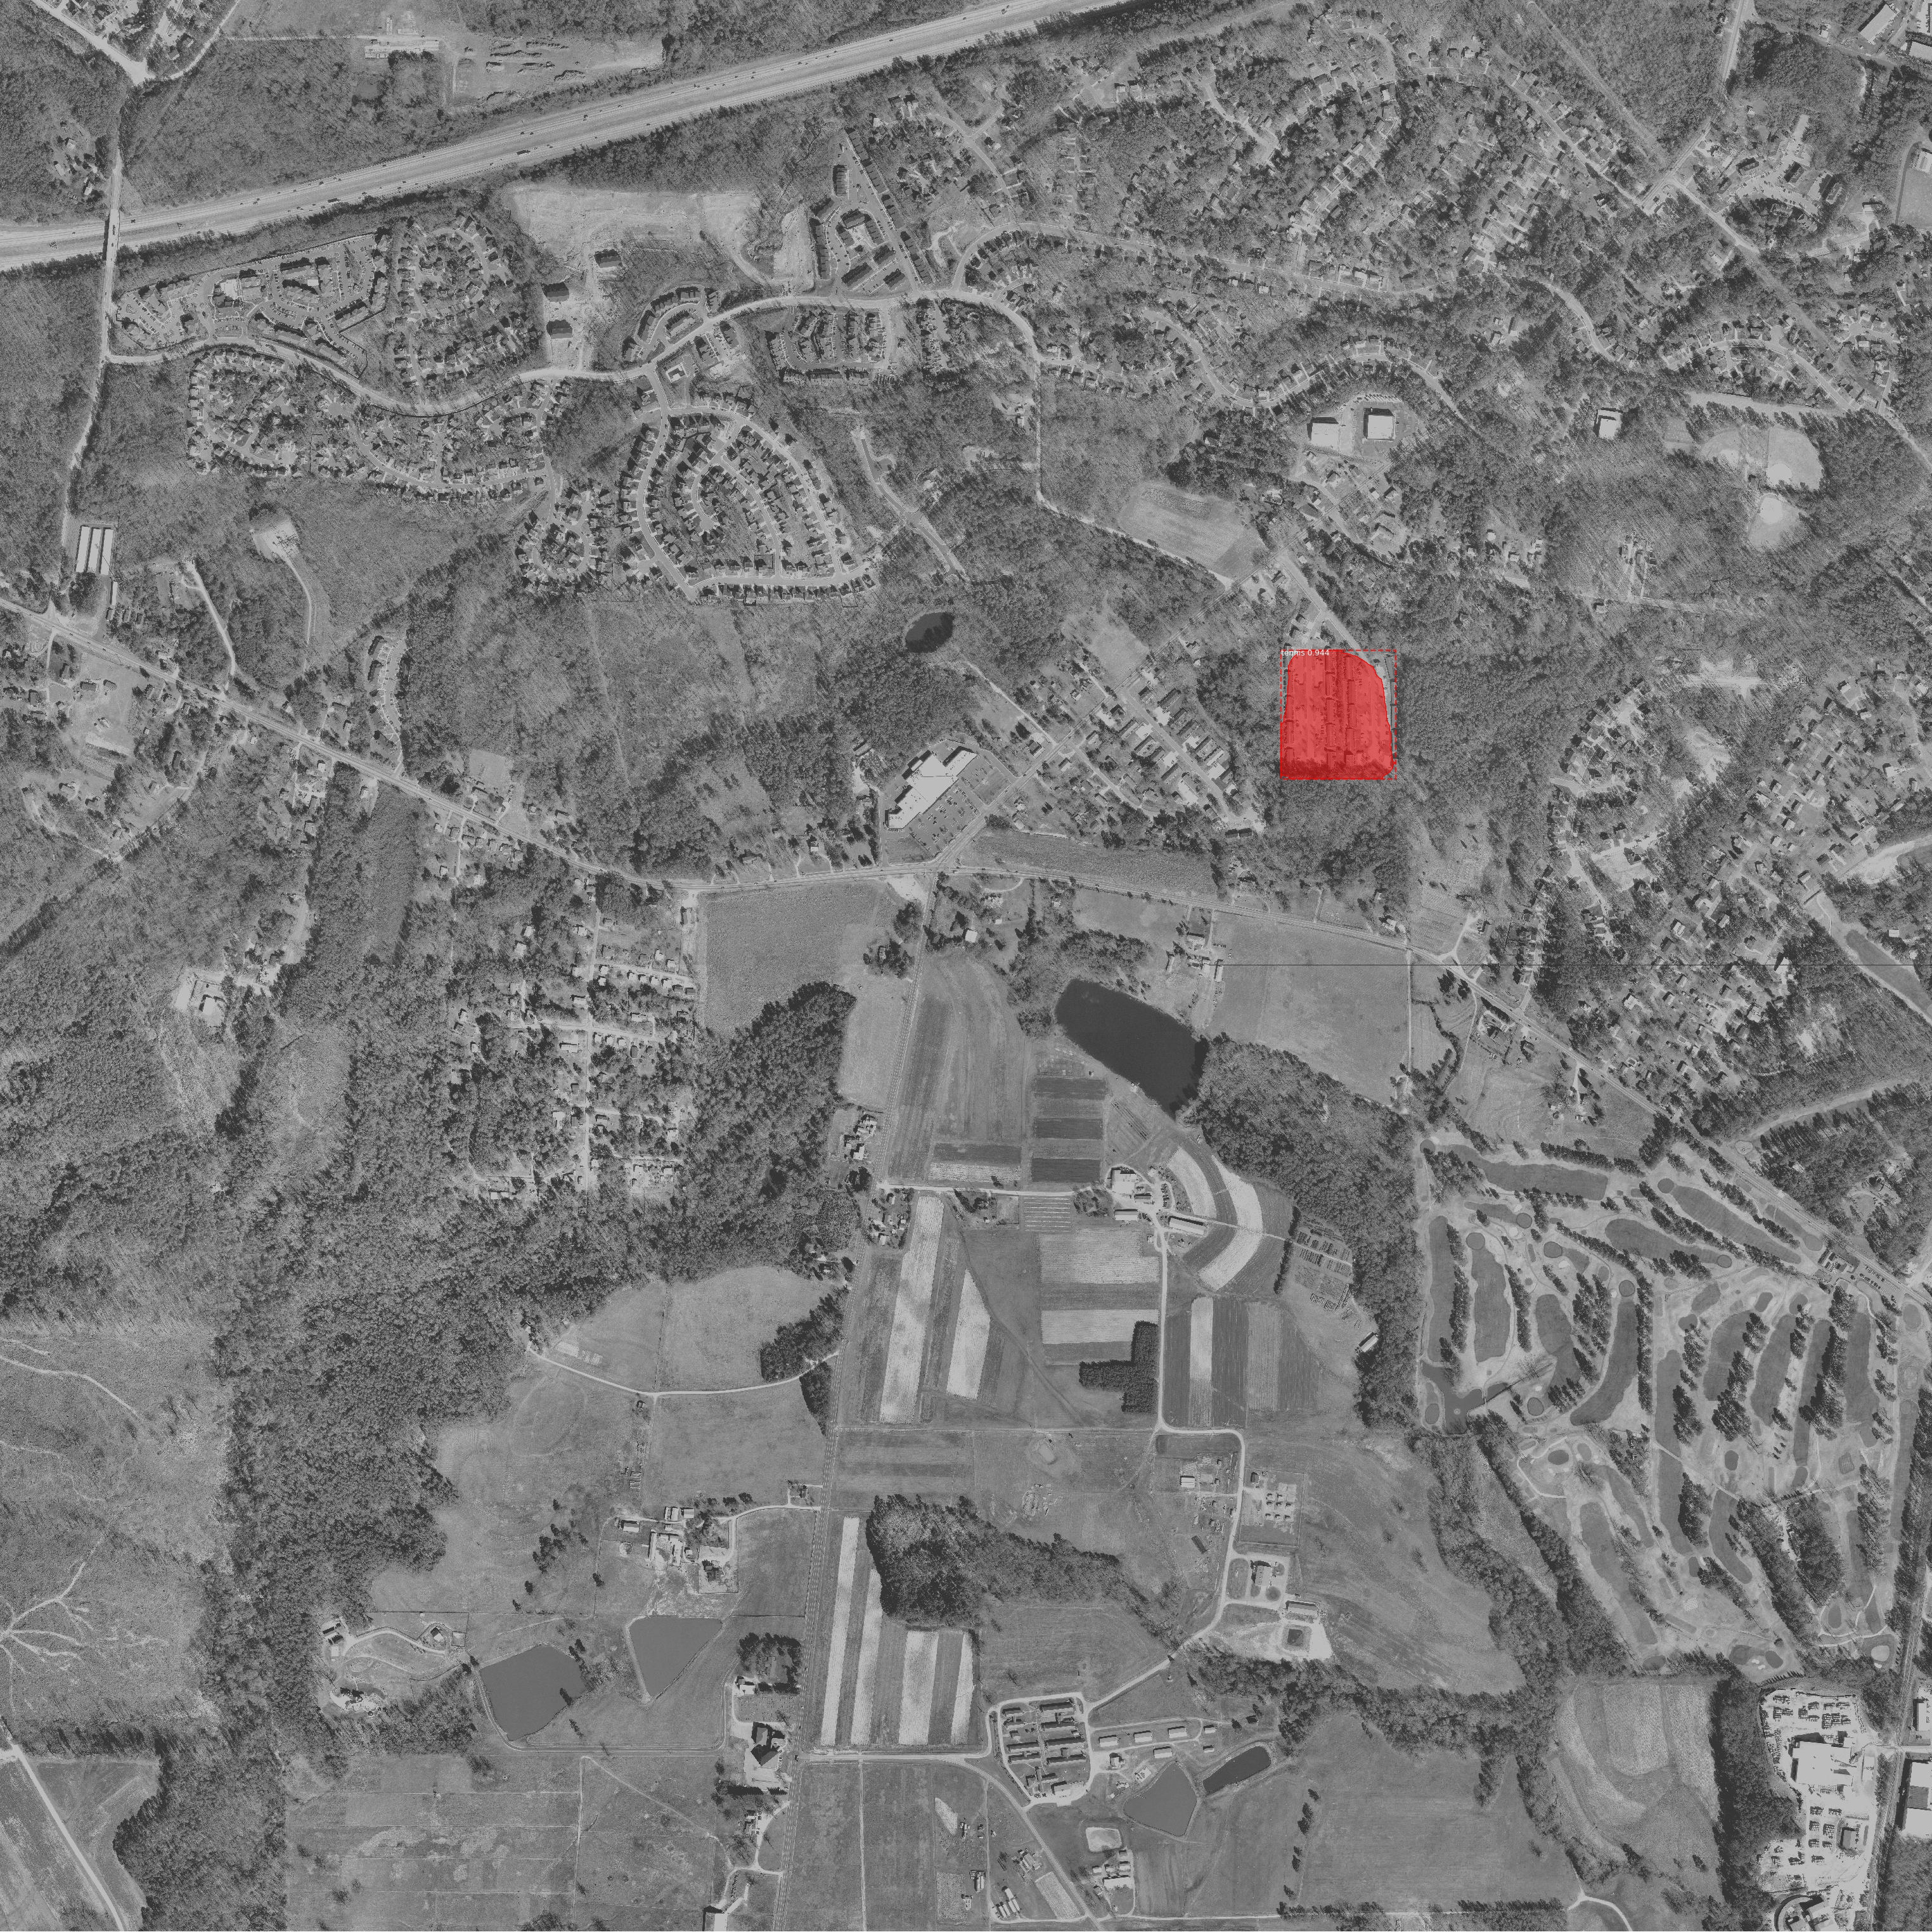
\includegraphics[width=.4\linewidth]{3}}
\hfill
\subfigure[Georeferenced polygons (GRASS output without background)]{\includegraphics[width=.4\linewidth]{4}}
\hfill
\end{figure}
% Your document ends here!
\end{document}